\vspace{-0.1cm}

Naive Bayes (henceforth NB) and Logistic Regression (henceforth LogReg) classifiers are among the most popular first choices for large scale text classification problems in the industry.
We use the Naive Bayes classifier over multinomial distribution with Dirichlet prior of $1.0$ as a baseline.
This baseline has also been the choice baseline in \cite{Shen12, Sun14} for categorizing product titles at scale due to its low runtime requirements.
Naive Bayes classifier is a specialization of Logistic Regression classifier \cite{Ng01}, where the latter is much more insensitive to dataset imbalance due to optimization of log-odds ratios in the objective function and much more so in the presence of effective regularizers such as L1 and Elastic Net \cite{ESL03, Zhang04:SGD, Zou05:EN}.
We refrain from using a KNN classifier due to our very high dimensional feature spaces which can lead to prohibitively long prediction times under arbitrary feature transforms even under an efficient KD-Tree data structure \cite{Manning08:IR}.

\vspace{-0.2cm}
\subsection{Data Preprocessing}
\label{Subsect:Data-preprocessing}
\vspace{-0.2cm}

Our data preprocessing steps are minimal.
For each listing, our primary text data is the product title. 
For AmazonJ and BU2 datasets, we also extract the list price whenever available. 
Additionally for BU2 dataset, we add the leaf node of navigational breadcrumbs, whenever available, as another meta feature.
BU1 dataset only has titles.
From every such listing, we remove standard English stopwords and tokens that appear in 10 listings or less i.e. rare tokens. 
We have found out that this removal reduces vocabulary sizes by almost 50\% without reducing classification performance.
We however, do not remove stopwords for the CNN classifier.
Instead to reduce vocabulary size for CNN, we replace rare tokens by the nominal token ``[RARE]'' and all numbers by the nominal form ``[NUM]''.
Further, all text is lowercased.
In all prediction experiments, we do not consider classes with less than 10 listings for test evaluation -- those classes are only used for training.

\vspace{-0.1cm}
\subsection{Initial Experiments with Business Unit 1 dataset}
\label{Subsect:BU1-exp}

\begin{wrapfigure}{l}{0.71\textwidth}
	\vspace{-0.8cm}
	\centering
	\subfloat[{Prediction on 10\% test set using word unigram count features}]{\label{Figure_BU1-WUC}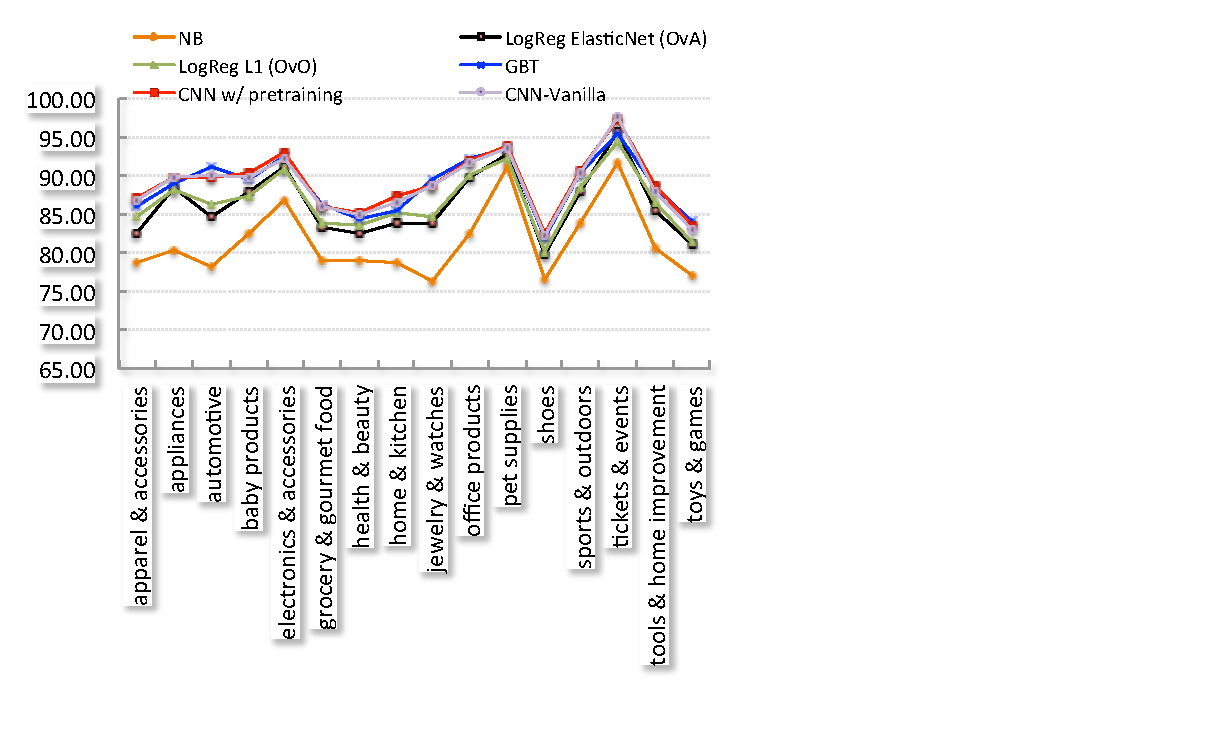
\includegraphics[width=0.35\textwidth]{images/BU1-WUC-predictions}} \hspace{0.05cm}
	\subfloat[{Prediction on 10\% test set using word unigram bi-positional count features}]{\label{Figure_BU1-WUBPC}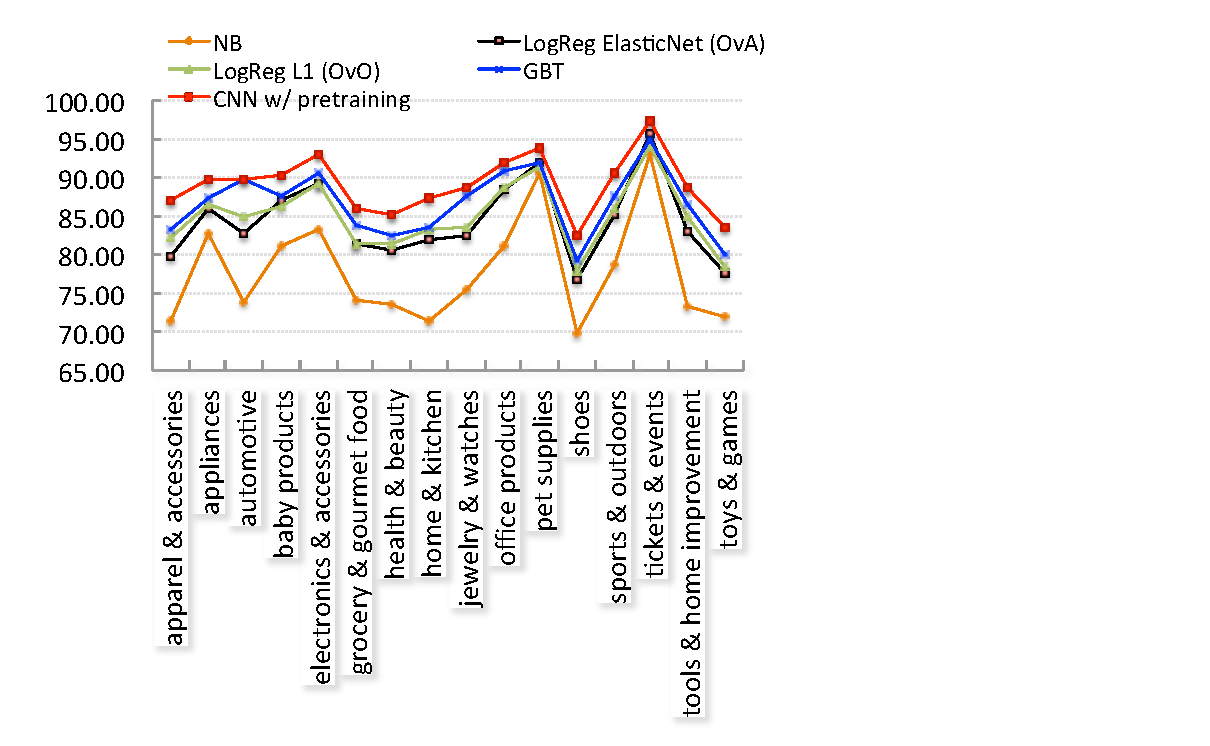
\includegraphics[width=0.35\textwidth]{images/BU1-WUBPC-predictions}} 

	\subfloat[{Prediction on 10\% test set using word bigram count features}]{\label{Figure_BU1-WBC}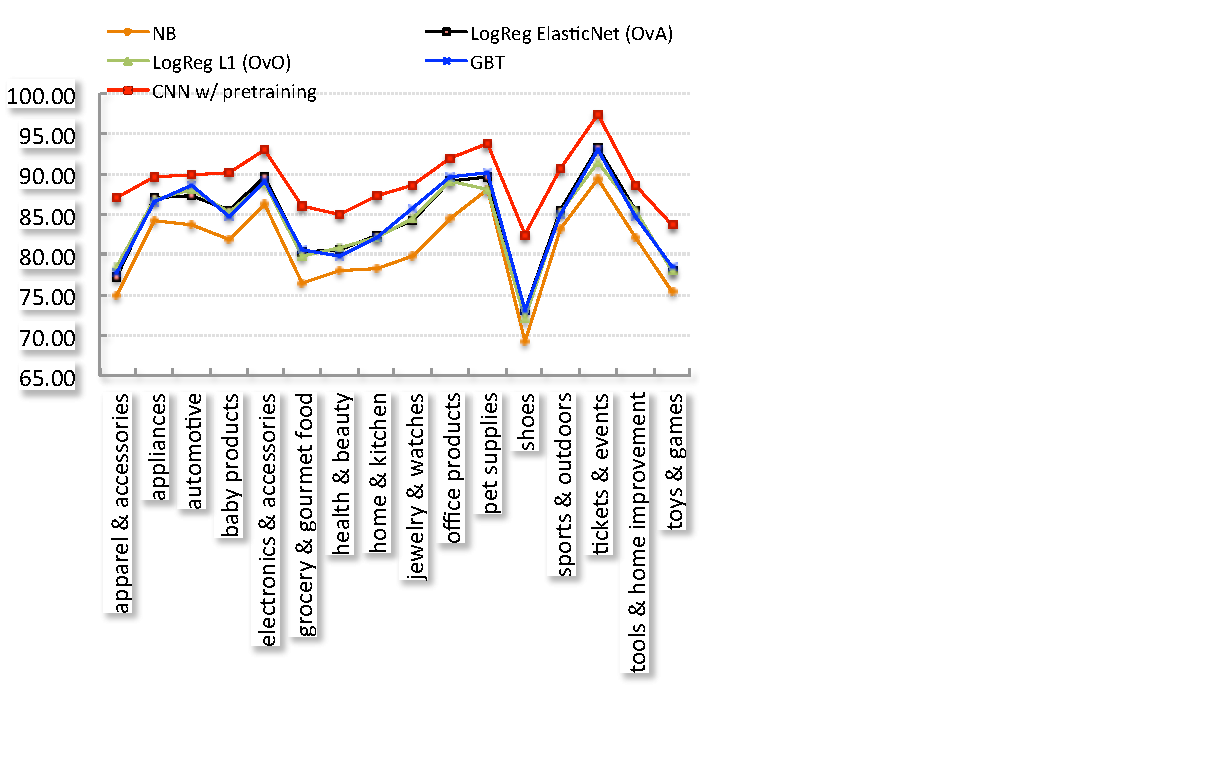
\includegraphics[width=0.35\textwidth]{images/BU1-WBC-predictions}} \hspace{0.05cm}
	\subfloat[{Prediction on 10\% test set using word bigram bi-positional count features}]{\label{Figure_BU1-WBBPC}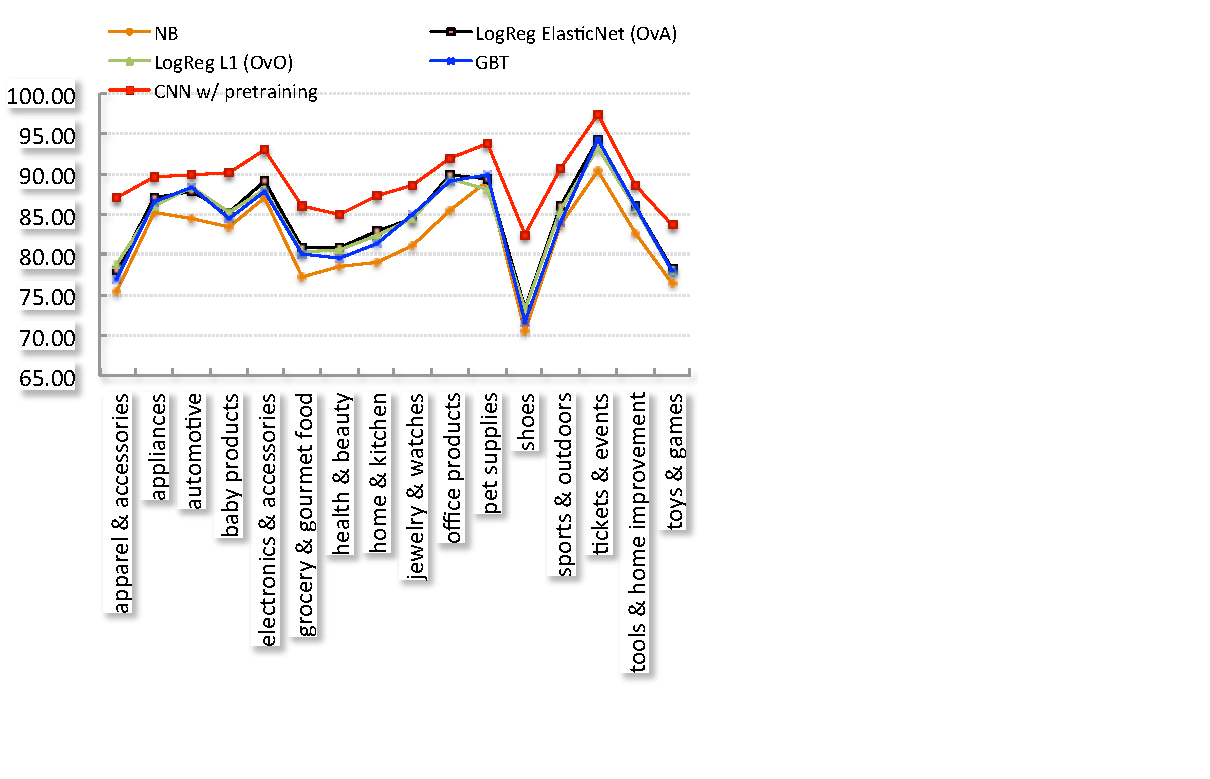
\includegraphics[width=0.35\textwidth]{images/BU1-WBBPC-predictions}} 
	\caption{\small{Predictions on BU1 test set for different classifiers. The CNN classifier has only one configuration and thus shows constant curves in all plots. Best viewed in color.} }
	\label{Figure_BU1-predictions}
	\vspace{-0.3cm}
\end{wrapfigure}
Our initial experiments with NB also consisted of using three other features -- a word bigram feature, a bi-positional word unigram feature and a bi-positional word bigram feature.
Consider a title text ``\textit{120gb hd 5400rpm sata fdb 2 5 mobile}'' from the ``\textbf{Data storage}'' leag node of Electronics taxonomy subtree and another title text ``\textit{acer aspire v7 582pg 6421 touchscreen ultrabook 15 6 full hd intel i5 4200u 8gb ram 1tb hdd 20gb ssd nvidia geforce gt 720m}'' from the ``\textbf{Laptops and netbooks}'' leaf node of the same subtree.
For bi-positional features, we split the length of the title in half and augment word uni/bi-grams with a left/right-half position. It was observed that some merchants would put laptop specific words up front and storage and peripheral specific words later for the listings in ``Laptops'' leaf node while the opposite for listings in ``Data storage'' leaf node.
This educated guess did help NB significantly (Fig. \ref{Figure_BU1-predictions-feature-averages}) but not the other classifiers.
For feature values, we use the feature descriptor counts within the title, except that of list price whose value we use directly (with rounding in NB classifier).
In the legends in all figures henceforth, ``OvO'' means ``One vs. One'' and ``OvA'' means ``One vs All''; L1 means L1 regularization \cite{LibLinear} and ElasticNet \cite{Zou05:EN} is a linear combination of 15\% L1 regularization and 85\% L2 regularization.
\begin{wrapfigure}{r}{0.45\textwidth}
	\vspace{-0.6cm}
	\centering
	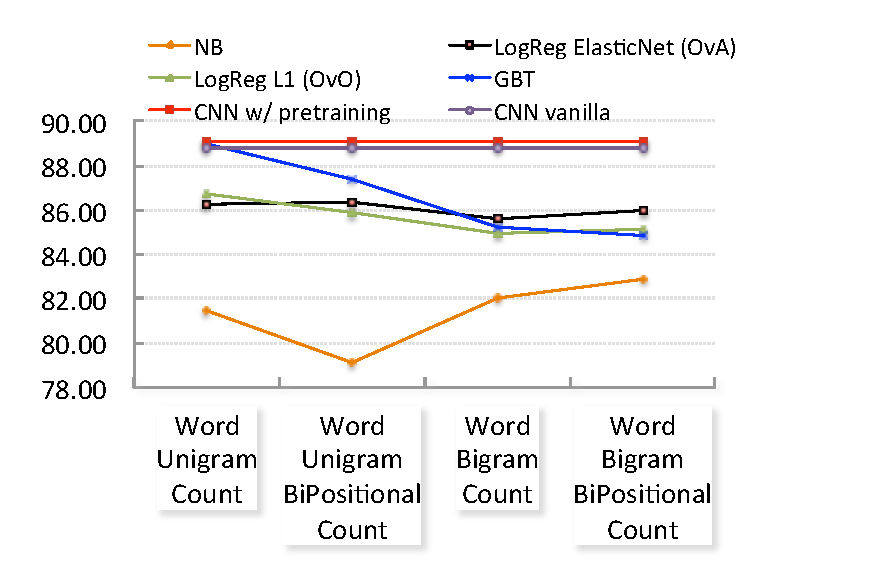
\includegraphics[width=0.43\textwidth]{images/BU1-mean-micro-precision}
	\caption{\small{Mean micro precisions of different classifiers over different feature setups except CNN.}}
	\label{Figure_BU1-predictions-feature-averages}
	\vspace{-0.4cm}
\end{wrapfigure}
For CNN experiments, we use an adaptation of TensorFlow \cite{TensorFlow}.

We observe from Figs. \ref{Figure_BU1-WUC}, \ref{Figure_BU1-WUBPC}, \ref{Figure_BU1-WBC} and \ref{Figure_BU1-WBBPC} that word unigram count features perform very well except NB and we decide to use this feature in all of our subsequent experiments.
Additionally, the micro precisions (and F1s) of CNN and GBT are statistically significant than the other classifiers for BU1 dataset over word unigrams under a paired t-test with a p-value $<$ at least $0.0001$. 
%% TODO: Pew Putthividya POS ??


\subsection{Classification Improvements with List Price on BU2 Dataset}
\label{Subsect:BU2-classification-improve-list-price}


Word unigram features have proved to be very effective for GBTs. 
However, improvements in classification performance have been observed for the BU2 dataset when we include the list price and leaf nodes of the navigational breadcrumbs when available. 
BU1 dataset has neither of these.
We experiment with a smaller taxonomy subtree of ``\textit{Women's Clothing}'' consisting of $\approx2.85$ million deduplicated listings. 

\begin{wrapfigure}{l}{0.43\textwidth}
	\vspace{-0.5cm}
	\centering
	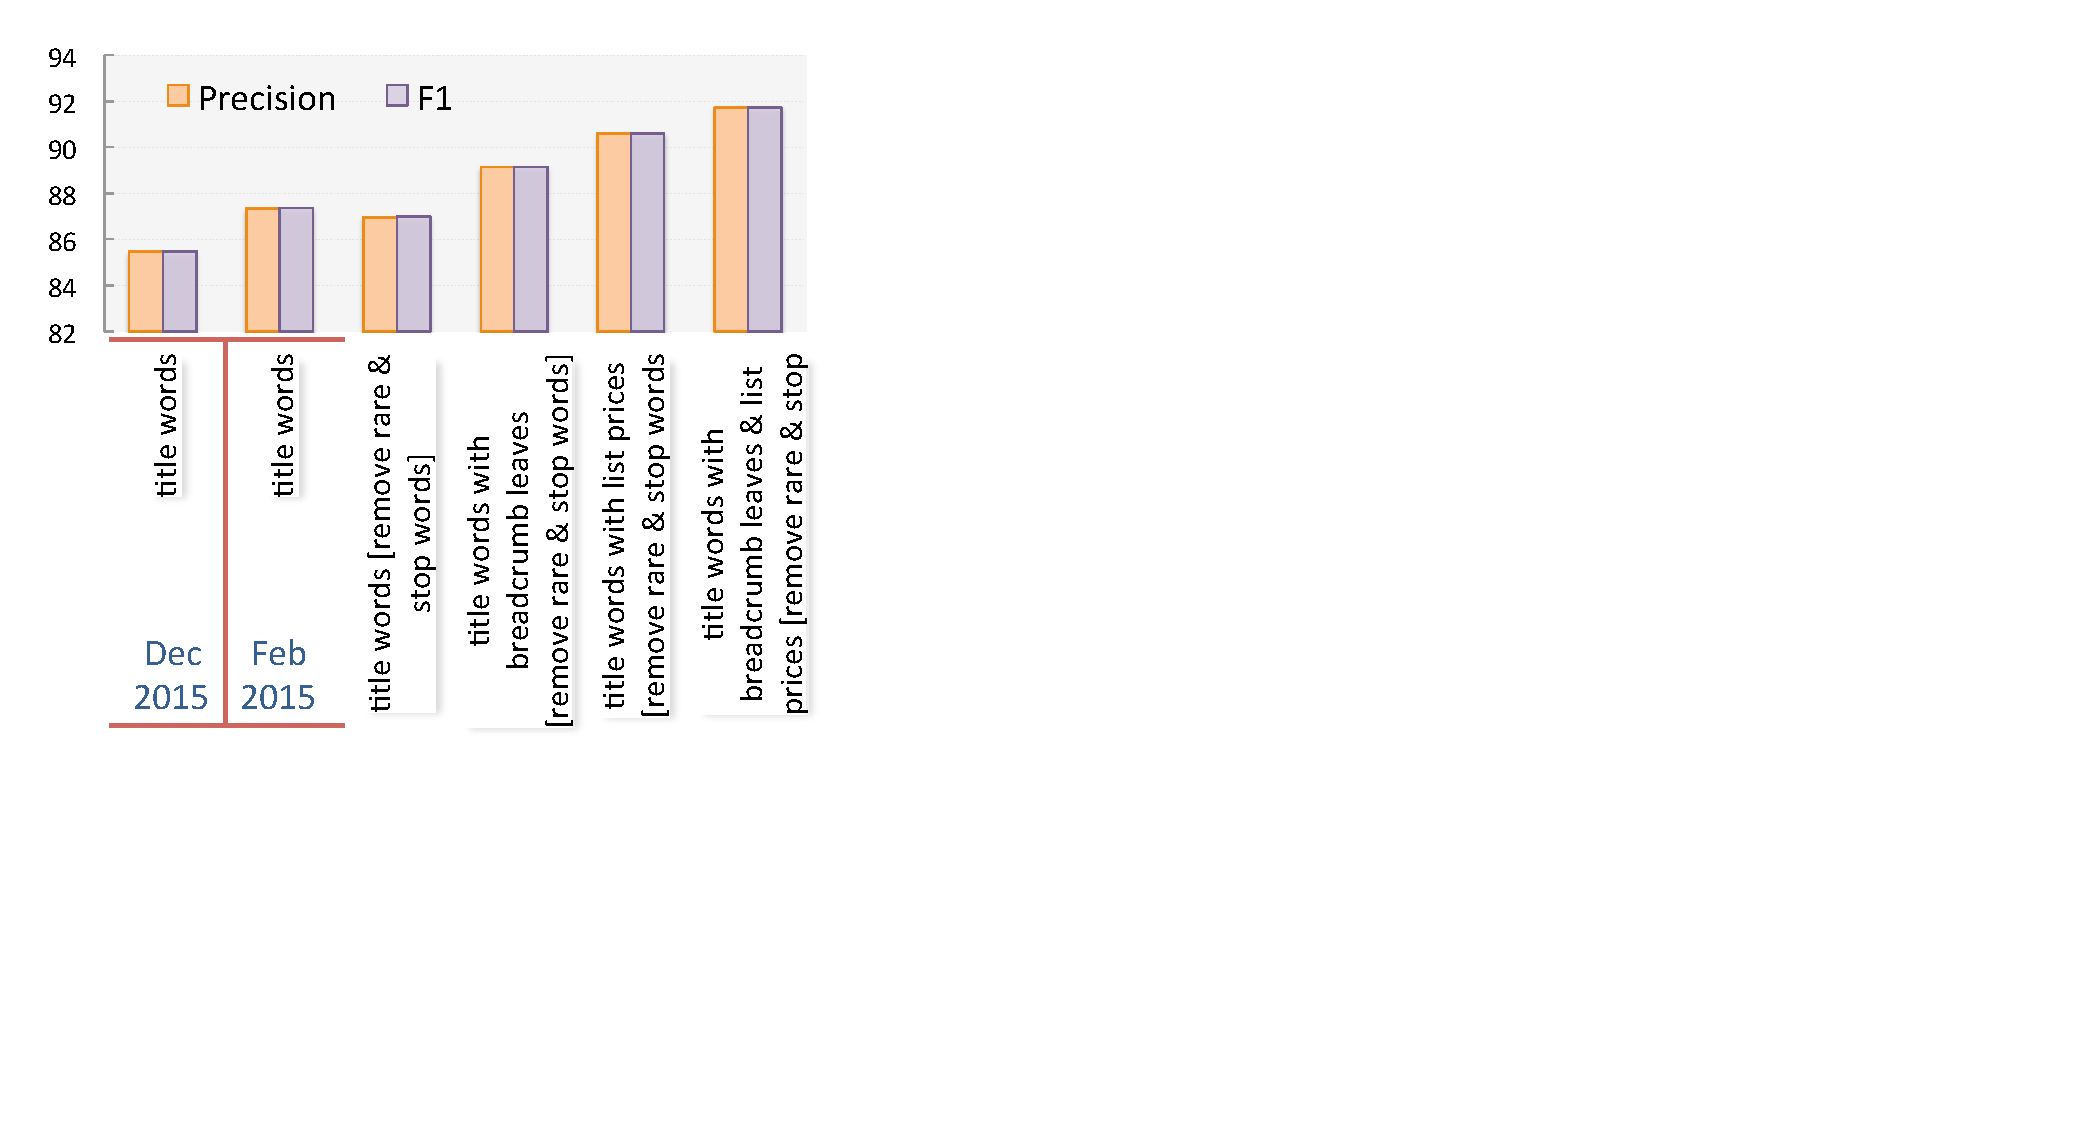
\includegraphics[width=0.43\textwidth]{images/BU2-gbt-feature-improvements}
	\caption{Improvements in micro precision and F1 of GBTs over different feature sets on the Women's Clothing subtree from BU2}
	\label{Figure_BU2-gbt-feature-improvements}
	\vspace{-0.4cm}
\end{wrapfigure}
The graph to the left of the vertical red line in Fig. \ref{Figure_BU2-gbt-feature-improvements} show the micro precision and F1 for the Women's Clothing subtree derived from the Dec 2015 40 million deduplicated data snapshot.
The graphs to the right of the red line show improvements in the classification performance due to the removal of stopwords and rare words and addition two types of meta features.
Further, the graphs to the right of the red line are obtained from subtree derived from the Feb 2016 204 million deduplicated data snapshot.
Clearly, the set of features corresponding to the last bar graph in Fig. \ref{Figure_BU2-gbt-feature-improvements} prove to be advantageous and we use these features for the AmazonJ dataset as well when available for all classifiers except CNN.
All of these numbers are before any cleaning of the BU2 dataset which we describe briefly in the next section.
The second bar graph in Fig. \ref{Figure_BU2-gbt-feature-improvements} emphasizes the fact that more training data benefits a classifier.

\subsection{Noise Analysis of Business Unit 2 Dataset using Correspondence LDA}
\label{Subsect:BU2-noise-analysis}

 
\begin{wrapfigure}{r}{0.7\textwidth}
	\vspace{-0.4cm}
	\centering
	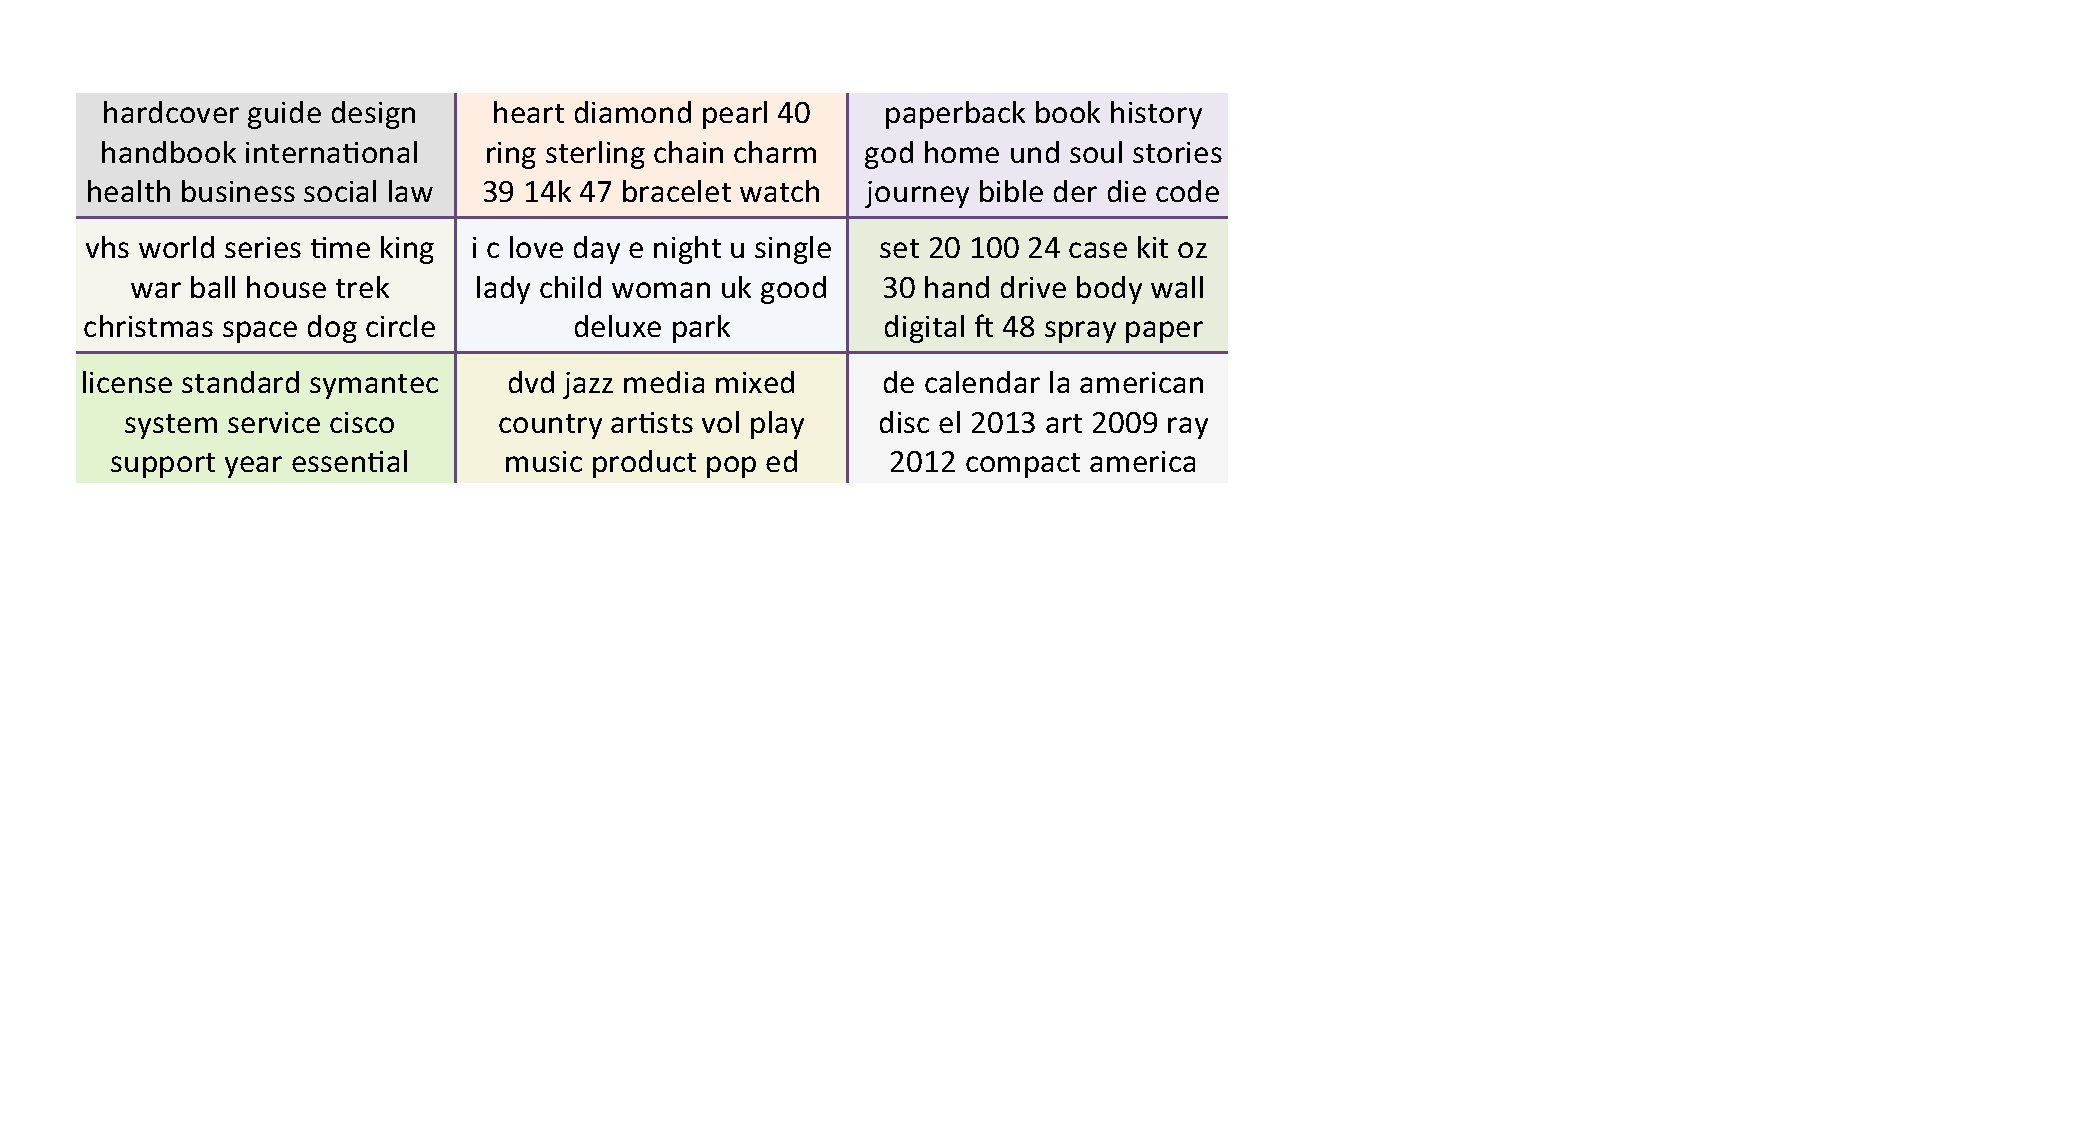
\includegraphics[width=0.7\textwidth]{images/BU2-noise-topics}
	\vspace{-0.4cm}
	\caption{{Latent ``noise'' topics over listings in \textbf{Shoes} taxonomy subtree.}}
	\label{Figure_BU2-noise-topics}
	\vspace{-0.3cm}
\end{wrapfigure}
The problem of low micro precision of $\approx65\%$ for the top level Shoes subtree in Fig. \ref{Figure_BU2-WUC-LogRegL1} has initially led us to think that label flips in the vendor's datasets might be to blame.
Motivated by the fact that the labels $\bm{y}$ might be misleading to compute $p(\bm{y}|\bm{x})$ and impossibility to manually verify even a representative subset of over 34 million listings for shoes alone in the 204 million Feb 2016 dataset snapshot, we sought to compute $p(\bm{x})$ over latent classes $z_k$ i.e. topics.

We use the CorrMMLDA model in \cite{Das11} due to its lower perplexity.
The number of topics has been set to 100 which is roughly double the number of branches for the Shoes subtree.	
The correspondence view consists of the words in the title and the content view consists of brands (when available) and merchant names. 
This is due to the fact that for a listing, the store and brand words are distributions over title words that in turn are distributions over latent $z_k$s.
 
\begin{wrapfigure}{r}{0.65\textwidth}
	\vspace{-0.5cm}
	\centering
	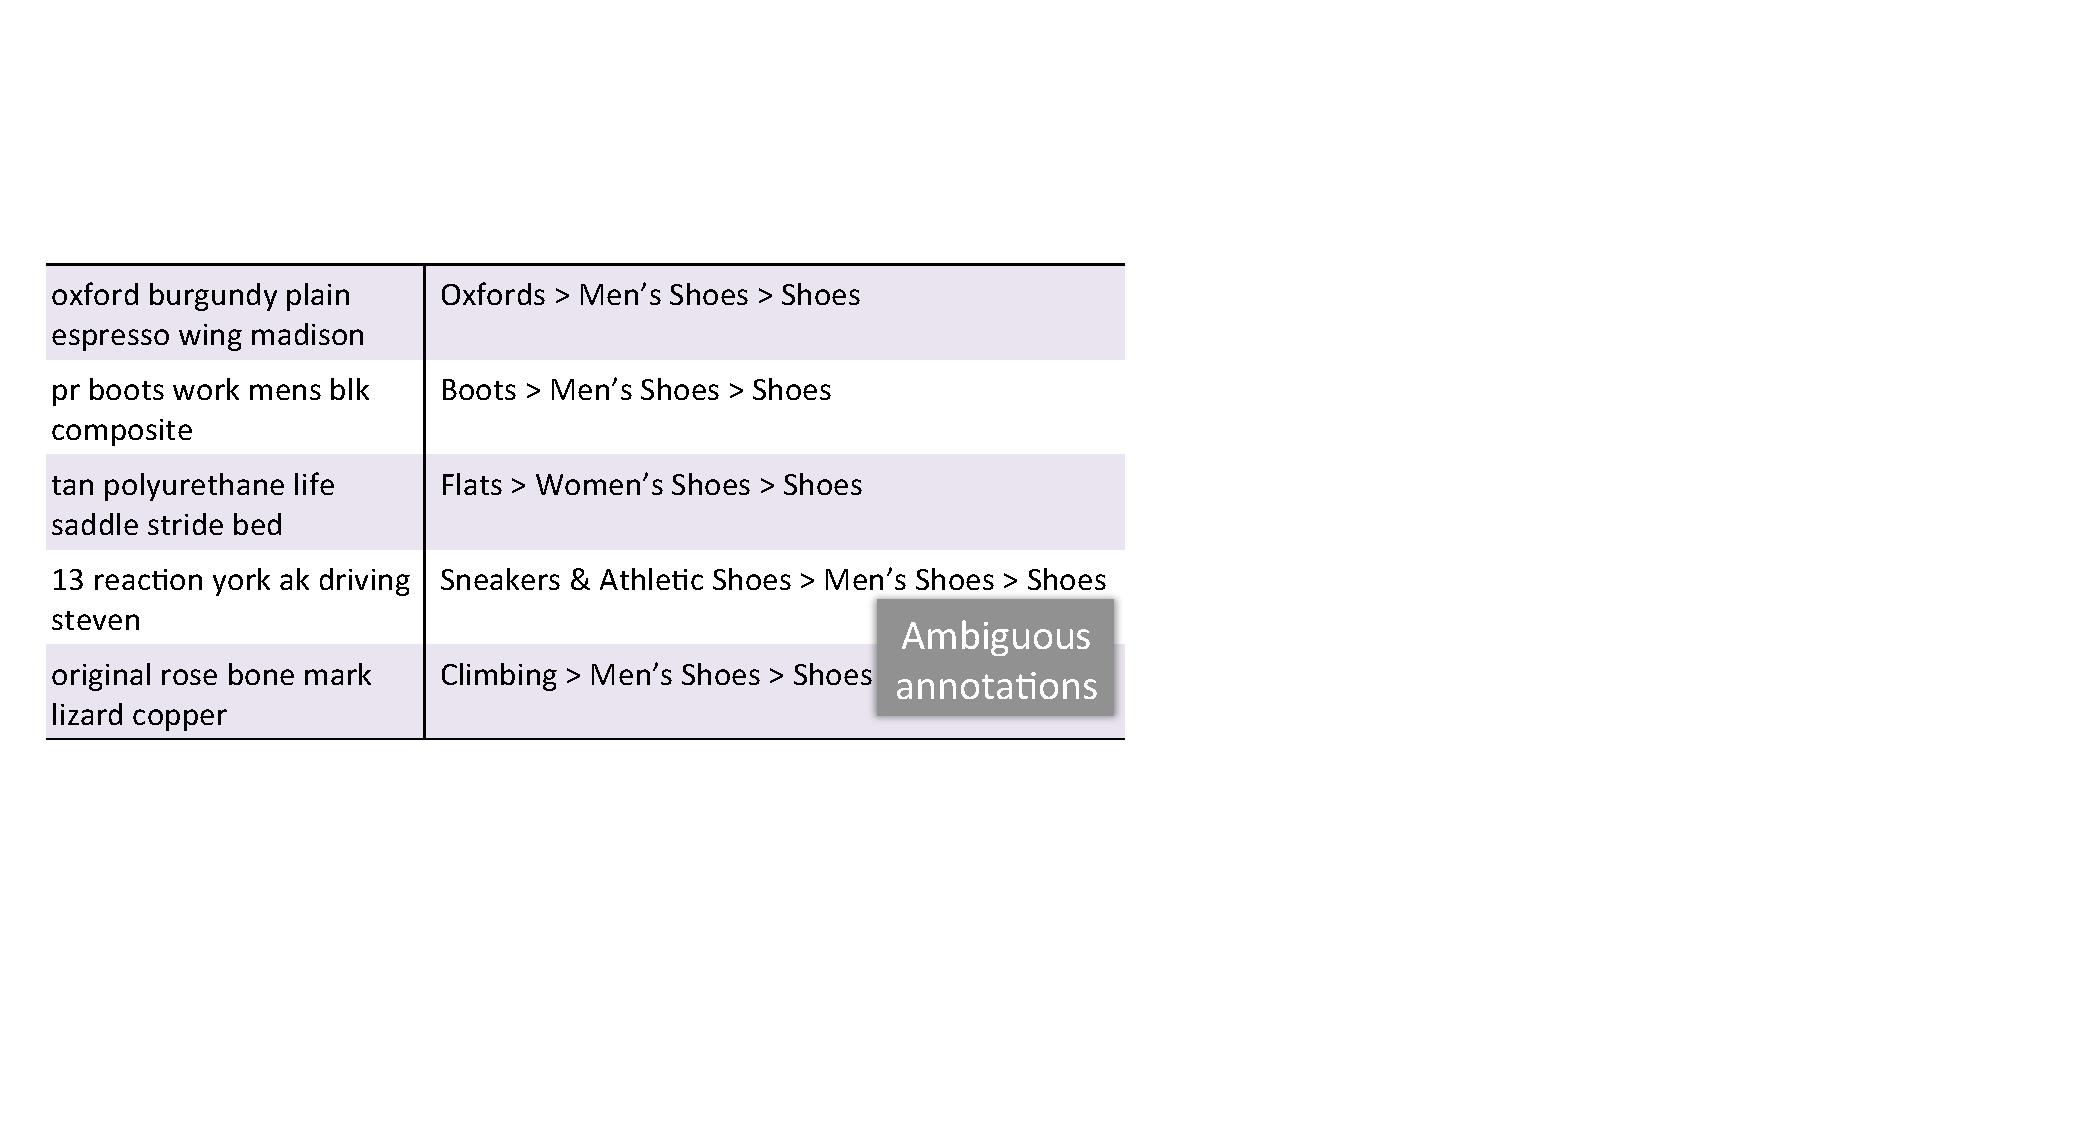
\includegraphics[width=0.65\textwidth]{images/BU2-topic-annotation}
	\vspace{-0.4cm}
	\caption{\small{Interpretation of latent topics using predictions from a GBT classifier. The topics here are excluding those in Fig. \ref{Figure_BU2-noise-topics}. Topics are from Feb 2016 snapshot.}}
	\label{Figure_BU2-topic-annotation}
	\vspace{-0.3cm}
\end{wrapfigure}
A sample of nine latent topics in Fig. \ref{Figure_BU2-noise-topics} clearly show that the most probable words over those topics are easily judged to be outside of the \textit{Shoes} domain.
Further, we also annotate the top six words (average length of titles in Shoes) of the latent topics using a GBT model trained over the initial and noisy Shoes listings. 
Human judges tried to verify if the annotations from GBT in Fig. \ref{Figure_BU2-topic-annotation} indeed describe the latent topic descriptions.
While most of the annotated topic annotations make sense, several topics such as the bottom two rows in Fig. \ref{Figure_BU2-topic-annotation} are ambiguous.

We next uniformly sample hundred listings from each of the irrelevant and ambiguous topics and manually inspect the listings. 
For the BU2 dataset, it has been found that listings from many out-of-domain merchants got included as part of the Shoes listings owing to a supposedly inaccurate blackbox categorization module from the data vendor.
Fortunately, for BU2 dataset, the vendor's mistakes has been consistent and this allowed us to manually inspect only the list of all 277 merchants for all listings in the top level fifteen taxonomy subtrees and remove listings corresponding to the out-of-domain ones.
One can think of this latter activity analogous to manual rule creation in \cite{Sun14}.
After this aggressive cleaning the average number of merchants per subtree dropped to X from Y.
The number of deduplicated listings also dropped from 204 million to 60 million in total for BU2 dataset.

In summary, we have been able to clean more than a third of the listings by manually inspecting $K\times10$ to $K\times20$ most probable words from the $K$ topics and $J\times100$ listings instead of 204 million of them with $J << K$.
One major advantage of using the technique discussed above is that automatic annotations of latent topics (Fig. \ref{Figure_BU2-topic-annotation}) can be used to create an initial taxonomy automatically using some other external taxonomy on the same category. 
For example, if BU2 needs to visualize a specific taxonomy of Food that does not currently exist, they can use topic modeling of their listings on Food together with automatic labeling of the topics using a classifier trained on the Food subtree from BU1.


\vspace{-0.2cm}
\subsection{Minimal Parameter Tuning of Classifiers}
\label{Subsect:experimental_setup>param_tuning}
\vspace{-0.2cm}

We fine tune the parameters of the classifiers using 10\% development set of the Apparel/Clothing categories of the datasets and apply the same configuration to all of the other subtree specific classifiers.
This reduced experimentation time for more expensive classifiers such as GBT and CNN.

\clearpage
